\documentclass[11pt, a4paper]{article}

% ─── Packages ────────────────────────────────────────────────────────────────
\usepackage[margin=1in]{geometry}
\usepackage{amsmath, amssymb}
\usepackage{booktabs}
\usepackage{graphicx}
\usepackage{array}
\usepackage{multirow}
\usepackage{caption}
\usepackage{subcaption}
\usepackage{hyperref}
\usepackage{parskip}
\usepackage[T1]{fontenc}
\usepackage{lmodern}
\usepackage{xcolor}
\usepackage{enumitem}

\hypersetup{colorlinks=true, linkcolor=black, urlcolor=blue, citecolor=black}

% ─── Title ───────────────────────────────────────────────────────────────────
\title{%
  \textbf{Sentiment Analysis on Amazon Product Reviews}\\[0.4em]
  \large A Comparative Study of LSTM and BERT\\[0.2em]
  \normalsize CS6120 Natural Language Processing --- Team 102
}
\author{Xuyang Shen \quad Yu Ye\\
  \small Northeastern University}
\date{March 2026}

% ─────────────────────────────────────────────────────────────────────────────
\begin{document}
\maketitle
\tableofcontents
\vspace{0.5em}\hrule\vspace{1em}

% ─────────────────────────────────────────────────────────────────────────────
\section{Introduction}
% ─────────────────────────────────────────────────────────────────────────────

Sentiment analysis --- the task of automatically identifying the emotional polarity of natural language text --- is one of the most practically impactful problems in NLP. In this project, we apply sentiment analysis to Amazon Software product reviews, converting user star ratings into binary sentiment labels (positive / negative) and independently training two architecturally distinct models: a Long Short-Term Memory (LSTM) network with static GloVe embeddings, and a pre-trained BERT transformer fine-tuned for sequence classification.

The central research question is: \textbf{to what extent does pre-training on large corpora and dynamic contextual representations explain performance differences over a traditional LSTM baseline, particularly under severe class imbalance?}

Both models are trained on identical data splits to ensure a controlled comparison. The results reveal a striking divergence not captured by accuracy alone --- a divergence best illustrated by their respective confusion matrices. Sections 2--5 describe each model independently; Section 6 provides the joint comparative analysis.

% ─────────────────────────────────────────────────────────────────────────────
\section{Dataset}
% ─────────────────────────────────────────────────────────────────────────────

We use the Amazon Product Reviews dataset (Software category) provided by He \& McAuley \cite{mcauley2016ups}. The raw dataset consists of user reviews with associated star ratings (1--5). Following standard practice \cite{zhang2018deep}, we convert ratings to binary sentiment labels: 4--5 stars $\rightarrow$ \textbf{Positive} (1), 1--2 stars $\rightarrow$ \textbf{Negative} (0). Three-star reviews are excluded as they represent ambiguous neutral sentiment.

\begin{table}[h]
\centering
\caption{Dataset Statistics}
\begin{tabular}{lrr}
\toprule
\textbf{Split} & \textbf{Samples} & \textbf{Ratio} \\
\midrule
Train      & 8,964 & 80\% \\
Validation & 1,121 & 10\% \\
Test       & 1,121 & 10\% \\
\midrule
\textbf{Total} & \textbf{11,206} & \\
\bottomrule
\end{tabular}
\end{table}

\textbf{Class Imbalance.} The binary label distribution is highly skewed: approximately 80.2\% of reviews are positive (4--5 stars) and only 19.8\% are negative (1--2 stars). This imbalance reflects the natural distribution of Amazon review ratings, where five-star reviews account for the majority of user-submitted content \cite{mcauley2016ups}. This imbalance is a critical challenge for both models, though each handles it differently.

% ─────────────────────────────────────────────────────────────────────────────
\section{LSTM Model (Xuyang Shen)}
% ─────────────────────────────────────────────────────────────────────────────

\subsection{Data Preprocessing}

The LSTM pipeline preprocesses raw text through the following steps: (1) lowercase conversion and punctuation removal; (2) stopword filtering using the NLTK English stopword corpus to remove non-informative tokens; (3) whitespace tokenization. Three-star reviews were excluded prior to splitting.

A vocabulary of \textbf{16,199 words} was built from the training set (minimum word frequency $\geq 2$). Pre-trained GloVe embeddings (300-dimensional, 6B token corpus \cite{pennington2014glove}) were used to initialize a fixed embedding matrix. Each vocabulary word was mapped to its corresponding GloVe vector; out-of-vocabulary tokens were initialized with a random normal distribution ($\sigma = 0.6$). The embedding layer was subsequently frozen during training.

\subsection{Model Architecture}

\begin{table}[h]
\centering
\caption{LSTM Architecture}
\begin{tabular}{lll}
\toprule
\textbf{Layer} & \textbf{Configuration} & \textbf{Notes} \\
\midrule
Embedding       & $16{,}199 \times 300$  & GloVe weights, frozen \\
LSTM (2 layers) & hidden dim $= 256$     & \texttt{batch\_first}, dropout $= 0.5$ \\
Dropout         & $p = 0.5$              & Applied to final hidden state \\
Linear          & $256 \rightarrow 1$    & Classification head \\
Sigmoid         & ---                    & Binary probability output \\
\bottomrule
\end{tabular}
\end{table}

The embedding layer is frozen to prevent overfitting on the limited 10K-sample training set. The final hidden state of the last LSTM layer, $\mathbf{h}_T^{(2)}$, is passed through dropout and a linear layer, producing a scalar probability for binary classification.

\subsection{Training}

\begin{table}[h]
\centering
\caption{LSTM Training Hyperparameters}
\begin{tabular}{ll}
\toprule
\textbf{Hyperparameter} & \textbf{Value} \\
\midrule
Optimizer       & Adam \\
Learning rate   & $1 \times 10^{-3}$ \\
Loss function   & Binary Cross Entropy (\texttt{BCELoss}) \\
Batch size      & 64 \\
Max epochs      & 10 \\
Early stopping  & patience $= 3$, monitor: validation loss \\
Hardware        & Apple MPS \\
\bottomrule
\end{tabular}
\end{table}

The best validation loss ($\approx 0.497$) was achieved at Epoch 4. Training was halted at Epoch 7 by early stopping as validation performance continued to deteriorate. The optimal weights were restored prior to evaluation.

\begin{figure}[h]
  \centering
  
\includegraphics[width=0.62\textwidth]{loss_curves.png}
  \caption{LSTM Training and Validation Loss over Epochs}
  \label{fig:lstm_loss}
\end{figure}

\subsection{Results}

\begin{table}[h]
\centering
\caption{LSTM Test Set Metrics}
\begin{tabular}{ll}
\toprule
\textbf{Metric} & \textbf{Value} \\
\midrule
Accuracy  & 80.37\% \\
Precision & 80.50\% \\
Recall    & 99.67\% \\
F1-Score  & 0.8907  \\
\bottomrule
\end{tabular}
\end{table}

\begin{table}[h]
\centering
\caption{LSTM Confusion Matrix}
\begin{tabular}{cc|cc}
\toprule
 & & \multicolumn{2}{c}{\textbf{Predicted}} \\
 & & Negative & Positive \\
\midrule
\multirow{2}{*}{\textbf{Actual}}
  & Negative & \textbf{5}   & 217 \\
  & Positive & 3            & \textbf{896} \\
\bottomrule
\end{tabular}
\label{tab:lstm_cm}
\end{table}

% ─────────────────────────────────────────────────────────────────────────────
\section{BERT Model (Yu Ye)}
% ─────────────────────────────────────────────────────────────────────────────

\subsection{Data Preprocessing \& Tokenization}

Unlike the LSTM pipeline, BERT does not require manual text cleaning. The raw review text is fed directly to the \texttt{bert-base-uncased} WordPiece tokenizer, which handles lowercasing, subword splitting, and the insertion of special tokens (\texttt{[CLS]}, \texttt{[SEP]}) automatically. Each input is padded or truncated to a maximum length of 256 tokens, determined via exploratory data analysis of the review length distribution. An attention mask is passed alongside each input to ensure padding tokens do not contribute to self-attention computation.

\subsection{Model Architecture}

The model is \texttt{BertForSequenceClassification} (\texttt{bert-base-uncased}) with a 2-class linear head appended on top of the \texttt{[CLS]} token representation. The base model comprises 12 transformer encoder layers, 12 attention heads per layer, and a hidden dimension of 768, for a total of \textbf{109,483,778 parameters} (all trainable during fine-tuning).

\begin{table}[h]
\centering
\caption{BERT Architecture Summary}
\begin{tabular}{ll}
\toprule
\textbf{Property} & \textbf{Value} \\
\midrule
Base model       & \texttt{bert-base-uncased} \cite{devlin2019bert} \\
Layers           & 12 transformer encoder blocks \\
Attention heads  & 12 per layer \\
Hidden dim       & 768 \\
Total parameters & 109,483,778 \\
Classification   & Linear head on \texttt{[CLS]} token \\
\bottomrule
\end{tabular}
\end{table}

\subsection{Training}

\begin{table}[h]
\centering
\caption{BERT Training Hyperparameters}
\begin{tabular}{ll}
\toprule
\textbf{Hyperparameter} & \textbf{Value} \\
\midrule
Optimizer            & AdamW (weight decay $= 0.01$) \\
Learning rate        & $2 \times 10^{-5}$ \\
LR scheduler         & Linear warmup + linear decay \\
Warmup steps         & 10\% of total training steps \\
Gradient clipping    & max norm $= 1.0$ \\
Batch size           & 16 \\
Epochs               & 4 \\
Hardware             & T4 GPU (Google Colab) \\
\bottomrule
\end{tabular}
\end{table}

\begin{figure}[h]
  \centering
  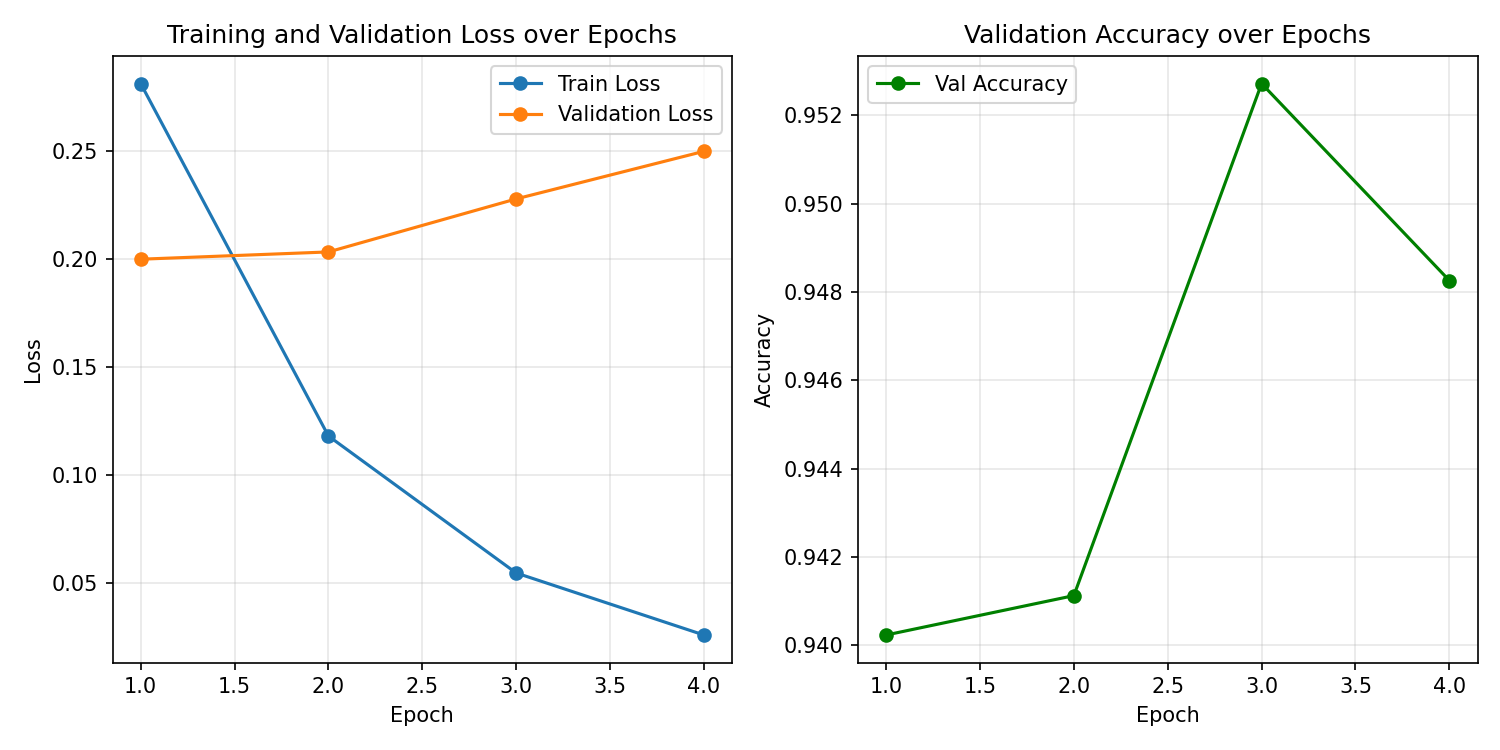
\includegraphics[width=0.8\textwidth]{bert_loss_curves.png}
  \caption{BERT Training/Validation Loss and Validation Accuracy over Epochs}
  \label{fig:bert_loss}
\end{figure}

\subsection{Results}

\begin{table}[h]
\centering
\caption{BERT Test Set Metrics}
\begin{tabular}{ll}
\toprule
\textbf{Metric} & \textbf{Value} \\
\midrule
Accuracy           & 93.84\% \\
Precision          & 94.82\% \\
Recall (Positive)  & 97.66\% \\
Recall (Negative)  & 78.38\% \\
F1-Score           & 0.9622 \\
\bottomrule
\end{tabular}
\end{table}

\begin{figure}[h]
  \centering
  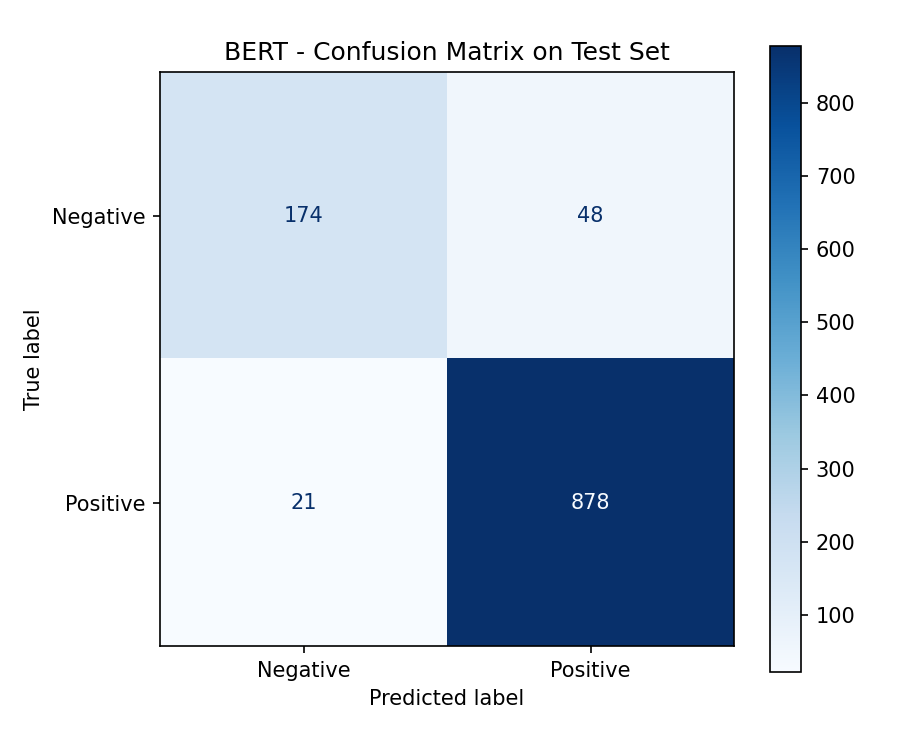
\includegraphics[width=0.52\textwidth]{bert_confusion_matrix.png}
  \caption{BERT Confusion Matrix on Test Set}
  \label{fig:bert_cm}
\end{figure}

% ─────────────────────────────────────────────────────────────────────────────
\section{Comparative Analysis}
% ─────────────────────────────────────────────────────────────────────────────

\subsection{Overall Performance}

\begin{table}[h]
\centering
\caption{LSTM vs.\ BERT --- Test Set Performance Summary}
\begin{tabular}{lrrrrrr}
\toprule
\textbf{Model} & \textbf{Acc.} & \textbf{Prec.} & \textbf{Rec. (+)} & \textbf{Rec. ($-$)} & \textbf{F1} & \textbf{Size} \\
\midrule
LSTM (GloVe)       & 80.37\% & 80.50\% & 99.67\% &  2.25\% & 0.8907 & $\sim$5 MB \\
BERT (fine-tuned)  & 93.84\% & 94.82\% & 97.66\% & 78.38\% & 0.9622 & 417.6 MB \\
\midrule
$\Delta$ (BERT$-$LSTM) & \textbf{+13.47\%} & \textbf{+14.32\%} & $-2.01\%$ & \textbf{+76.13\%} & \textbf{+0.0715} & --- \\
\bottomrule
\end{tabular}
\end{table}

BERT outperforms the LSTM baseline across all aggregate metrics. The most significant gap, however, is not in accuracy or F1 --- it is in \textbf{negative class recall} (+76.13 percentage points). This difference exposes a fundamental failure mode in the LSTM that aggregate metrics conceal.

\subsection{Confusion Matrix Analysis: Two Models, Opposite Failure Modes}

\begin{table}[h]
\centering
\caption{Side-by-Side Confusion Matrices}
\begin{tabular}{c|cc|cc}
\toprule
 & \multicolumn{2}{c|}{\textbf{LSTM Predicted}} & \multicolumn{2}{c}{\textbf{BERT Predicted}} \\
\textbf{Actual} & Neg. & Pos. & Neg. & Pos. \\
\midrule
Negative (222) & \textbf{5}   & 217 & \textbf{174} & 48  \\
Positive (899) & 3            & \textbf{896} & 21  & \textbf{878} \\
\bottomrule
\end{tabular}
\label{tab:cm_compare}
\end{table}

The confusion matrices reveal that the two models do not merely differ in performance level --- they exhibit \textbf{structurally opposite error patterns}.

The LSTM produces 217 False Positives and only 3 False Negatives. In other words, it correctly identifies 896 of 899 positive reviews (99.67\% recall) but captures only 5 of 222 negative reviews (2.25\% recall). From a decision-theoretic perspective, the LSTM has effectively learned a degenerate strategy: predict positive for nearly every input. This is not the result of poor architecture per se, but of the interaction between a flat loss function and severe class imbalance.

BERT, by contrast, produces 48 False Positives and 21 False Negatives --- a much more balanced error profile. It still favors the positive class (positive recall 97.66\% vs. negative recall 78.38\%), but the asymmetry is far less extreme. Critically, BERT identifies 174 of 222 negative reviews correctly --- a 34$\times$ improvement over the LSTM's 5.

\subsection{Why Does BERT Handle Class Imbalance Better?}

A natural question is: why does BERT fare so much better on the minority class, given that \textit{neither model applies any explicit class weighting}? The explanation lies in the quality and origin of the learned representations.

\textbf{Pre-training as implicit data augmentation.} BERT is pre-trained on approximately 3.3 billion tokens using masked language modeling \cite{devlin2019bert}. During this process, it encounters vast numbers of negative-sentiment expressions (complaints, disappointment, criticism) across many domains. When fine-tuned on our 10K Amazon dataset --- which contains only $\sim$1,780 negative training examples --- BERT can leverage this pre-existing semantic knowledge to recognize negative sentiment even from sparse supervision. The LSTM, starting from GloVe vectors and random LSTM weights, must learn this from scratch.

This generalizes Howard \& Ruder's finding \cite{howard2018ulmfit} that pre-trained language models outperform randomly-initialized architectures not just because of architecture, but because of \textit{knowledge transfer}: the pre-trained model has already ``seen'' the minority class in many guises across many corpora.

\textbf{Dynamic vs.\ static word representations.} GloVe assigns a single fixed vector to each word regardless of context \cite{pennington2014glove}. The word \textit{not} has the same embedding whether it precedes \textit{great}, \textit{terrible}, or \textit{refund}. The LSTM must learn to resolve negation and irony through its sequential hidden state --- a task that degrades as sequence length increases due to the vanishing gradient problem, even with gating mechanisms \cite{hochreiter1997lstm}.

BERT's self-attention mechanism directly models token-to-token interactions at every layer. Clark et al.\ \cite{clark2019what} showed that specific attention heads in BERT layers 8--12 consistently attend from negation words (\textit{not}, \textit{never}, \textit{barely}) to the sentiment-bearing words they modify. This behavior emerges from pre-training, not task-specific supervision, providing a principled mechanism for handling negation in product reviews --- precisely the linguistic pattern most common in low-star (negative) reviews.

\textbf{Optimizer and training stability.} The LSTM uses standard Adam with a fixed learning rate of $10^{-3}$. BERT uses AdamW \cite{loshchilov2017decoupled} with weight decay and a linear warmup scheduler, which warms the learning rate over the first 10\% of training steps before linearly decaying it. This prevents large gradient updates from destroying the pre-trained weights in early fine-tuning epochs --- an essential stability mechanism for large pre-trained models.

\subsection{An Interesting Analysis: Accuracy as a Misleading Metric}

The LSTM's 80.37\% accuracy appears competitive at first glance. However, a trivial majority-class classifier --- one that always predicts \textit{positive} --- would achieve exactly $\frac{899}{1121} \approx 80.2\%$ accuracy on this test set. The LSTM barely exceeds this baseline. Its reported accuracy is largely a product of the class prior, not learned discrimination.

This underscores a point frequently noted in the sentiment analysis literature \cite{zhang2018deep}: on imbalanced datasets, \textbf{macro-averaged F1 or per-class recall is a far more informative metric than accuracy}. The LSTM's F1 of 0.8907 is inflated by its near-perfect positive recall; its macro-F1 (averaging equally over both classes) would be significantly lower than BERT's.

\subsection{Efficiency vs.\ Performance Trade-off}

\begin{table}[h]
\centering
\caption{Computational Cost Comparison}
\begin{tabular}{lrr}
\toprule
\textbf{Aspect} & \textbf{LSTM} & \textbf{BERT} \\
\midrule
Parameters          & $\sim$4.4M              & 109.5M \\
Model size          & $\sim$5 MB              & 417.6 MB \\
Training time       & $<$ 5 min (CPU/MPS)     & 27.2 min (T4 GPU) \\
Required hardware   & CPU sufficient          & GPU required \\
Inference time      & Very fast               & $\sim$207 ms / batch of 16 \\
\bottomrule
\end{tabular}
\end{table}

BERT's performance advantage comes at a substantial computational cost. Training requires a dedicated GPU; inference latency is orders of magnitude higher than the LSTM. In resource-constrained deployment scenarios --- mobile applications, edge devices, or real-time streaming pipelines --- the LSTM may remain preferable despite its inferior discrimination ability. This reflects a genuine engineering trade-off that mirrors industrial practice \cite{zhang2018deep}.

% ─────────────────────────────────────────────────────────────────────────────
\section{Limitations and Future Work}
% ─────────────────────────────────────────────────────────────────────────────

\textbf{Class imbalance.} Neither model addressed the 80/20 class imbalance explicitly. For the LSTM, applying a weighted loss via \texttt{BCEWithLogitsLoss(pos\_weight=4.0)} would penalize false negatives on the minority class more heavily and is likely to substantially improve negative recall. For BERT, class-weighted cross-entropy or focal loss \cite{zhang2018deep} are established remedies.

\textbf{LSTM architecture.} Using a Bidirectional LSTM (BiLSTM) would allow the model to consider both left and right context when encoding each token, partially closing the gap with BERT's bidirectional attention \cite{zhang2018deep}.

\textbf{Dataset scale.} Our subset of 10K reviews is small by modern standards. Training the LSTM on the full Amazon dataset (millions of reviews) would provide substantially more negative examples and may reduce the majority-class collapse we observe.

\textbf{Aspect-level analysis.} Both models perform document-level sentiment classification. Amazon reviews often contain mixed sentiment (e.g., praising battery life while criticizing software quality). Aspect-based sentiment analysis \cite{sun2019utilizing} would produce richer and more actionable insights.

% ─────────────────────────────────────────────────────────────────────────────
\section{Conclusion}
% ─────────────────────────────────────────────────────────────────────────────

We trained and compared an LSTM with static GloVe embeddings and a fine-tuned BERT model on Amazon Software product review sentiment analysis. Both models achieve similar aggregate accuracy, but the confusion matrices reveal a qualitative difference: the LSTM effectively collapses to majority-class prediction (2.25\% negative recall), while BERT maintains meaningful discrimination across both classes (78.38\% negative recall).

We attribute this gap to three interacting factors: (1) BERT's pre-training provides rich semantic knowledge that transfers to the minority class even under sparse supervision; (2) dynamic contextual embeddings allow BERT to handle negation and irony that static GloVe vectors cannot represent; and (3) BERT's training recipe (AdamW, warmup scheduling, gradient clipping) provides stability absent in the LSTM setup.

These findings suggest that for real-world sentiment monitoring --- where detecting negative reviews is often more actionable than confirming positive ones --- pre-trained transformer models offer a qualitative advantage that aggregate metrics alone do not convey.

% ─────────────────────────────────────────────────────────────────────────────
\begin{thebibliography}{99}

\bibitem{devlin2019bert}
J.\ Devlin, M.-W.\ Chang, K.\ Lee, and K.\ Toutanova,
``BERT: Pre-training of Deep Bidirectional Transformers for Language Understanding,''
in \textit{Proc.\ NAACL-HLT}, 2019.

\bibitem{hochreiter1997lstm}
S.\ Hochreiter and J.\ Schmidhuber,
``Long Short-Term Memory,''
\textit{Neural Computation}, vol.\ 9, no.\ 8, pp.\ 1735--1780, 1997.

\bibitem{pennington2014glove}
J.\ Pennington, R.\ Socher, and C.\ Manning,
``GloVe: Global Vectors for Word Representation,''
in \textit{Proc.\ EMNLP}, 2014.

\bibitem{mcauley2016ups}
R.\ He and J.\ McAuley,
``Ups and Downs: Modeling the Visual Evolution of Fashion Trends with One-Class Collaborative Filtering,''
in \textit{Proc.\ WWW}, 2016.

\bibitem{howard2018ulmfit}
J.\ Howard and S.\ Ruder,
``Universal Language Model Fine-Tuning for Text Classification,''
in \textit{Proc.\ ACL}, 2018.

\bibitem{clark2019what}
K.\ Clark, U.\ Khandelwal, O.\ Levy, and C.\ D.\ Manning,
``What Does BERT Look At? An Analysis of BERT's Attention,''
in \textit{Proc.\ ACL Workshop BlackboxNLP}, 2019.

\bibitem{zhang2018deep}
L.\ Zhang, S.\ Wang, and B.\ Liu,
``Deep Learning for Sentiment Analysis: A Survey,''
\textit{WIREs Data Mining and Knowledge Discovery}, 2018.

\bibitem{sun2019utilizing}
C.\ Sun, L.\ Huang, and X.\ Qiu,
``Utilizing BERT for Aspect-Based Sentiment Analysis via Constructing Auxiliary Sentence,''
in \textit{Proc.\ NAACL-HLT}, 2019.

\bibitem{loshchilov2017decoupled}
I.\ Loshchilov and F.\ Hutter,
``Decoupled Weight Decay Regularization,''
in \textit{Proc.\ ICLR}, 2019.

\end{thebibliography}

\end{document}
